\chapter{Multi-ensemble atomic clocks with adaptive measurements}

This chapter describes work done towards implementation of multiple atomic ensembles and adaptive measurement techniques in an ion-based atomic clock. These methods were proposed in a paper by J. Borregaard and A. S. S\o rensen \cite{BorregaardSorensen} as a way to improve clock performance when the interrogating local oscillator (LO) is of limited quality. Implementing these methods in a lab-scale  system such as ours is a step towards realizing small-scale frequency references with suitably high performance. 

We will first discuss the basic principles of atomic frequency standards and how they are characterized. We will then review the aforementioned multi-ensemble and adaptive measurement methods proposed in Ref. \cite{BorregaardSorensen}. From there we will discuss the merits of implementing these methods in a $^{40}$Ca$^+$ based clock, and present a scheme for doing so (which is ultimately beyond the scope of this thesis). Finally, we will show preliminary results towards realizing this scheme, and discuss what steps should be taken next to continue this work. 





%%%%%%%%%%%%%%%%%%%%%%%%%%%

\section{Characterization of frequency standards}

An ideal frequency standard is a measurable periodic signal with a stable reference frequency $f_0$. Any signal generated by a real world device will inherently be subject to noise in both the measurement process and in the frequency of the oscillator \cite{RevModPhys.87.637}, resulting in an instantaneous signal frequency $f(t)$ which can waiver from $f_0$. Such a noisy signal can be written as \footnote{We ignore amplitude noise here.}
\begin{equation}  
A(t) = A_0 \sin{(2 \pi f_0 t + \phi (t))}
\end{equation}
where $\phi(t)$ represents fluctuations in the signal's phase away from the nominal phase $2 \pi f_0 t$. Instantaneous frequency drifts in a reference oscillator are generally described by the fractional frequency offset $y(t)$, which is proportional to $\dot{\phi} (t)$ \cite{FreqStands}:
\begin{equation}
y(t) = \frac{f(t) - f_0}{f_0} = \frac{1}{2 \pi f_0} \dot{\phi} (t) \, \text{.}
\label{eq:fracfreq}
\end{equation}
This implies that the average fractional frequency offset over some interval $\tau$ is
\begin{equation}
\bar{y} = \frac{1}{\tau} \int_{t}^{t + \tau}{y (t)} \ dt = \frac{1}{2 \pi f_0 \tau} ( \phi (t + \tau) - \phi (t) ) \ \text{.}
\label{eq:ybar}
\end{equation}
In this way, phase noise and frequency noise in the oscillator are directly related when we are considering the performance of a frequency standard. Measuring one gives us information about the other. 

In the frequency domain, the frequency stability of a reference oscillator is generally characterized by a power spectral density (PSD) function $S_y (f)$ of the function $y (t)$ (for frequencies $f \geq 0$). This function is typically modeled by a power law series which represents five specific noise types in the oscillator \cite{5570702,FreqStands}:
\begin{equation}
S_y (f) = h_{-2} f^{-2} + h_{-1} f^{-1} + h_{0} f^{0} + h_{1} f^{1} + h_{2} f^{2} 
\end{equation}
where $ h_{-2} f^{-2}$ represents random-walk frequency noise,  $h_{-1} f^{-1}$ represents flicker (aka pink) frequency noise, $h_{0} f^{0}$ represents white frequency noise, $h_{1} f^{1}$ represents flicker/pink phase noise, and $h_{2} f^{2}$ represents white phase noise. Fig. \ref{fig:PSDmodel} plots how $S_y (f)$ manifests for the different types of noise described. 

\begin{figure*}[tb]
    \begin{center}
        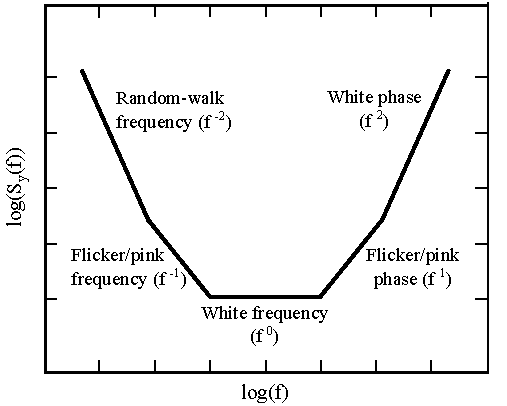
\includegraphics{figures/5/Fig_powerlaw}
        \caption{\label{fig:PSDmodel} Frequency noise power spectral density characteristics of a reference oscillator when modeled with power law series.}
    \end{center}
\end{figure*}

In the time domain, the frequency stability of a reference oscillator is generally derived from a set of successive measurements $\bar{y}_k$ over a common interval length $T$, where each $\bar{y}_k$ value is treated as a random variable. In this case, the standard metric for characterizing the time domain frequency stability of an oscillator is the two-sample Allan variance, defined as \cite{5570702, Allan}
\begin{equation}
\sigma_y^2 (\tau) = \frac{1}{2} \big\langle(\bar{y}_{k+1} - \bar{y}_k)^2 \big\rangle \ \text{.}
\end{equation}
The Allan variance assumes the simplest case of there being no (or negligible) dead time between measurements. It is worth noting that the Allan variance is a sample variance--it is estimated from a finite number two-sample variance values $\frac{1}{2} (y_{k+1} - y_k)^2$ which are averaged to obtain $\sigma_y^2 (T)$.


Atomic frequency standards use the energy splittings between the internal states of an atom, which are proportional to a frequency by Planck's constant, as a stable frequency reference. %For instance, the SI second  is officially defined as ''the duration of 9,192,631,770 periods of the radiation corresponding to the transition between the two hyperfine levels of the ground state of the caesium 133 atom.'' 
A reference atom, or ensemble of atoms, is interrogated by a local oscillator (LO) tuned near to the resonance frequency. The resulting signal from the resonant interaction can be measured and used to produce an error signal, which adjusts the noisy LO's frequency to best match the atomic frequency. This occurs periodically in intervals of $T_c$, such that the LO frequency remains matched to the reference frequency as best as can be accomplished over many intervals.

A common measurement scheme used to interrogate the atomic ensemble and produce the error signal  is the Ramsey method \cite{Rosenband, Ramsey}, which will be described in the next section. When using the Ramsey method, the standard quantum limit for the Allan variance becomes 
\begin{equation}
\sigma_y (\tau) = \sqrt{\sigma_y^2 (\tau)} = \frac{1}{2 \pi f_0 \sqrt{N T \tau}} \ \text{,}
\label{eq:shotlimit}
\end{equation}
where $N$ is the number of independent atoms in the ensemble and $\tau$ is the long-term averaging time \cite{Itano1993}. Beyond the choice of reference frequency $f_0$, the quantum limit in Eq. \ref{eq:shotlimit} is dependent on $N$, as well as the interrogation time $T$. Together these factors determine the limit of achievable performance in an atomic clock. 





%%%%%%%%%%%%%%%%%%%%%%%%%%%

\section{Ramsey interrogations in atomic clocks}

\begin{figure*}[hp]
    \begin{center}
        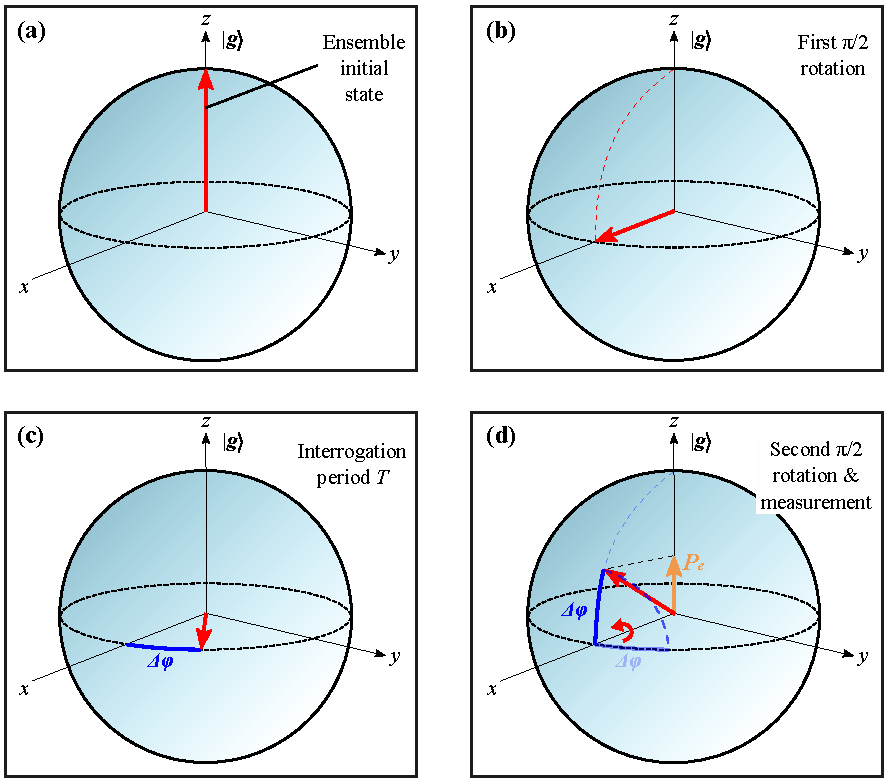
\includegraphics{figures/5/Fig_BlochRamsey}
        \caption{\label{fig:bloch} Ramsey measurement sequence illustrated in the Bloch sphere representation, which represents the 2-dimension complex Hilbert space in  Eq. \ref{eq:stateEvol}. (a) First, the initial atomic ensemble state (red arrow) is prepared in the ground state $|g \rangle$, corresponding to the z-axis of the Bloch sphere. (b) Second, the state is rotated 90$^{\circ}$ about the y-axis by a $\pi / 2$ pulse from the LO. (c) Third, the state free-evolves for the interrogation time $T$, accumulating phase $\Delta \phi$ from the noise in the LO. (d) Finally, the state is rotated 90$^{\circ}$ about the x-axis by a second $\pi / 2$ pulse, and $P_e$ is measured. Measurement projects the state onto the z-axis and carries an imprint of $\Delta \phi$ which can be used to produce the error signal for the clock. }
    \end{center}
\end{figure*}


Fig. \ref{fig:bloch} illustrates a Ramsey interrogation/measurement sequence in the Bloch sphere representation, which is a convenient visual representation of the 2-dimensional complex Hilbert space defining the time evolution in Eq. \ref{eq:stateEvol}. The measurement works as follows: First, the atomic ensemble to be interrogated is prepared in the ground state $|g\rangle = \begin{psmallmatrix} 1 \\ 0 \end{psmallmatrix}$. The atoms are then excited by the LO radiation at time $t$, for a duration $T_{\pi/2}$ such that $\Omega T_{\pi/2} = \pi / 2$ (where $\Omega$ is the coupling strength, as usual). We refer to these as $\pi/2$ pulses. The first pulse defines the phase between the LO and the atoms and leaves them in the state $\psi_1 = \frac{1}{\sqrt{2}} \begin{psmallmatrix}1 \\ -i \end{psmallmatrix}$, corresponding to a 90$^{\circ}$ rotation about the y-axis of the Bloch sphere\footnote{The axes are arbitrary until the phase between the LO and the atoms is defined by the first pulse.}. The atoms are then allowed to free-evolve for the interrogation period $T \gg T_{\pi/2}$. Any phase difference $\Delta \phi$ which accumulates between the noisy LO and the atoms during this time leaves them in the state $\psi_2 = \begin{psmallmatrix}1 & 0 \\ 0 & e^{-i \Delta \phi} \end{psmallmatrix} \psi_1$. Finally, at time $t + T$ the ensemble is given a second $\pi /2$ pulse, this time with a $\pi / 2$ phase shift in the LO relative to the first pulse. This corresponds to a 90$^{\circ}$ rotation about the x-axis of the Bloch sphere. A state detection is now made on the ensemble, giving
 $P_e(t+T) = N_e / N$ where $N_e$ is number of atoms projected into excited state $|e\rangle = \begin{psmallmatrix}0\\1 \end{psmallmatrix}$.

If $\Delta \phi = 0$ after the interrogation, then $\psi_1$ will have been recovered after the second $\pi / 2$ pulse, and $P_e(t+T) = 0.5$  (assuming perfect measurement). If $\Delta \phi \neq 0$ then the accumulated phase will be imprinted on the resulting measurement of $P_e(t+T)$. The purpose of phase-shifting the second $\pi / 2$ pulse is simply to maximize measurement sensitivity for small $\Delta \phi$.  From $\Delta \phi = \phi (t+T) - \phi (t)$ we may infer $\bar{y}$ for the interrogation interval, as per Eq. \ref{eq:ybar}, and produce the error signal. Any error or noise in the measurement process will also be imprinted on the LO--the probabilistic nature of the state measurement, for instance, leads to the $1/\sqrt{N}$ dependence in the quantum limit (Eq. \ref{eq:shotlimit}). Stochastic sources of error/noise will be averaged down over many cycles of the clock. %, as can be seen in Fig. TBD.


\begin{figure*}[t]
    \begin{center}
        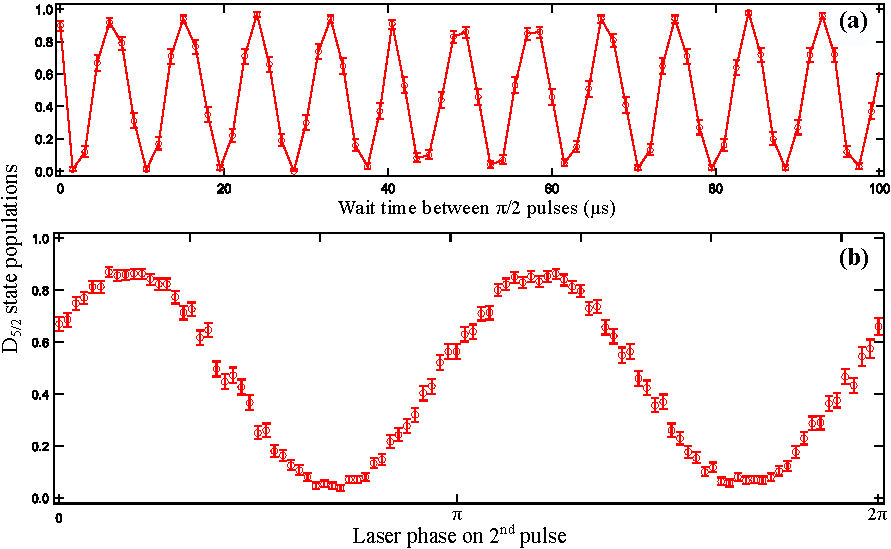
\includegraphics{figures/5/Fig_RamseyEx}
        \caption{\label{fig:RamseyEx} Two examples of Ramsey measurement data. (a) Ramsey measurements with varying interrogation times between the two $\pi / 2$ pulses. In this example, the second pulse was not shifted in phase relative to the first--this merely shifts the phase of the resulting data. The oscillations seen are due to the frequency detuning between the 729 nm laser and the ion (about 4 kHz in this instance). (b) Measurements made with no wait time between the two pulses, but with a varying phase in the second pulse. The purpose of the comparison is to demonstrate how a frequency difference between the LO and ion accumulates over time as a phase difference between the first and second pulses.
           }
    \end{center}
\end{figure*}

The measurement outcomes of a Ramsey sequence will take a $\sin^2$ profile in $\Delta \phi$; Fig. \ref{fig:RamseyEx} shows how this manifests in actual ion measurements. For clock operation, we are restricted to making measurements within the invertible region $|\Delta \phi| \leq \pi/2$. Beyond this range, the periodicity of the sinusoidal signal will result in degenerate measurements of $\bar{y}$, leading to significant over or under-corrections in the LO frequency that will degrade performance.






%%%%%%%%%%%%%%%%%%%%%%%%%%%%%%%%

\section{Improved LO stability with multiple atomic ensembles and adaptive measurements} 


\subsection{Clocks with multiple atomic ensembles}

The performance of an atomic clock is bound by the quantum limit in Eq. \ref{eq:shotlimit}. Because the reference frequency $f_0$ is fixed in a given clock, its best possible performance is dependent on the number of atoms $N$ and the interrogation time $T$. The number of atoms which can be practically implemented is usually limited by systematic factors. For instance, there may be electric field gradients over the spatial extent of large a ensemble cloud, or portions of the cloud which extend beyond the null of the RF trapping field. Uniformly addressing a large cloud with a gaussian optical beam can also be challenging. The interrogation time is limited by the necessity of measuring within the invertible region $|\Delta \phi| \leq \pi/2$. A noisier LO will accumulate phase more rapidly than a less noisy one, and will therefore have a more limited interrogation time. As such, the quality of the LO limits the long-term stability of a clock.

\begin{figure*}[ht]
   \begin{center}
        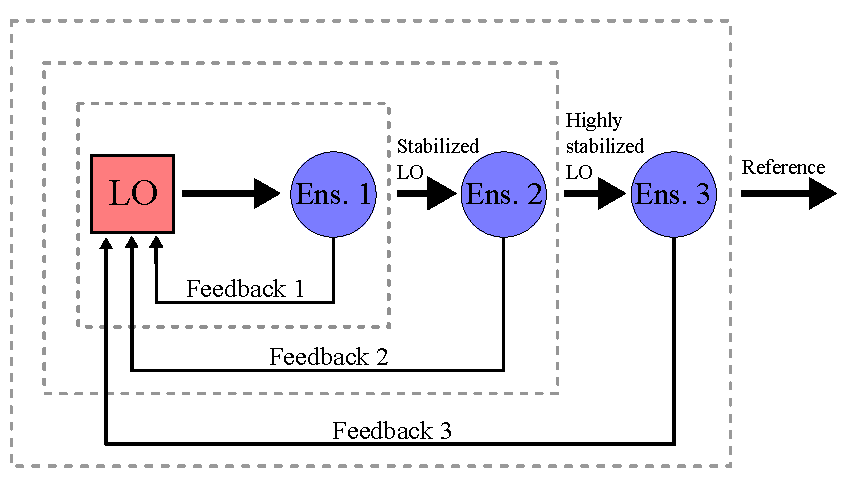
\includegraphics{figures/5/Fig_multiensembles}
        \caption{\label{fig:multiensemble} Illustration of locking the LO using multiple ensembles ($m = 3$, in this case). The first ensemble is interrogated for a time $T_1$ during the interrogation of the second and third ensembles. $T_1$ is sufficiently limited to keep the measurement within the invertible region $|\Delta \phi| \leq \pi/2$. Feedback from the first ensemble stabilizes the LO such that the second ensemble can be interrogated for $T_2 > T_1$. Feedback from the second ensemble further stabilizes the LO allows for $T_3 > T_2$, and so on. This method improves the stability of the clock by $N^{-(m/2)}$, where $m$ is the number of ensembles containing $N$ atoms each. }
    \end{center}
\end{figure*}


A proposal by Borregaard and S\o{}rensen \cite{BorregaardSorensen} describes novel methods by which interrogation times may be improved. First, they show that by locking the LO to several atomic ensembles instead of one, an improvement in stability (i.e. a decrease in $\sigma_y(\tau)$ in Eq. \ref{eq:shotlimit}) can be achieved which is proportional to $N^{-(m/2)}$, where $m$ is the number of ensembles containing $N$ atoms each. Fig. \ref{fig:multiensemble} illustrates how this method works. In essence, a single ensemble has a limited interrogation time $T_{1,max}$ due to the need to keep $\Delta \phi$ within the invertible region. If a second ensemble is interrogated simultaneously with $T_2 > T_{1,max}$, and the feedback from the first ensemble is used to correct the LO at some time $T_{1,max} < t < T_2$, then the $T_2$ interrogation of the second ensemble will not exceed the invertible region (within some limit $T_{2,max}$). The resulting correction from the second ensemble will provide a greater LO stabilization than would be achieved with regular measurement techniques. Adding subsequent ensembles to this feedback chain increases the resulting LO stability. For $m$ ensembles of $N$ ions each, the stability of the clock is, expressly,
\begin{equation}
\sigma_y (\tau) = \frac{1}{2 \pi f_0 \sqrt{\tau} } \frac{1}{(N \gamma \ T_{1,max})^{(m/2)}}  \sqrt{\gamma \ (\beta_1 / \beta)^{(m-1)} }
\label{eq:clockstab}
\end{equation}    
where $\gamma$ is a parameter characterizing the LO noise, and $\beta_1$ and $\beta$ are constants dependent on the noise spectrum of the uncorrected and corrected LO, respectively \cite{BorregaardSorensen}. Note that when $m = 1$, Eq. \ref{eq:shotlimit} is recovered.  


In Eq. \ref{eq:clockstab} we see that the clock stability is still limited by the maximum interrogation time of a single ensemble $T_{1,max}$, as well as the number of atoms per ensemble $N$. Simulations show that $\gamma T_{1,max} = 0.1$ is a limit above which improvement in the clock stability begins to be lost \cite{BorregaardSorensen}. For this upper value of $T_{1,max}$, ``break even'' improvement is achievable for as few as $N = 20$ atoms per ensemble in this protocol. Any fewer, and the resulting quantum projection noise from the first measurement injects too much noise into the second, such that the improvement becomes less than what would be achieved by simply having a single ensemble of $m N$ atoms. For $N_{min} = 20$, a factor of $\sim \sqrt{2^{(m-1)} }$ improvement in stability is predicted. 

%%%% 

\subsection{Adaptive measurement techniques in clock interrogations}


\begin{figure*}[ht]
    \begin{center}
        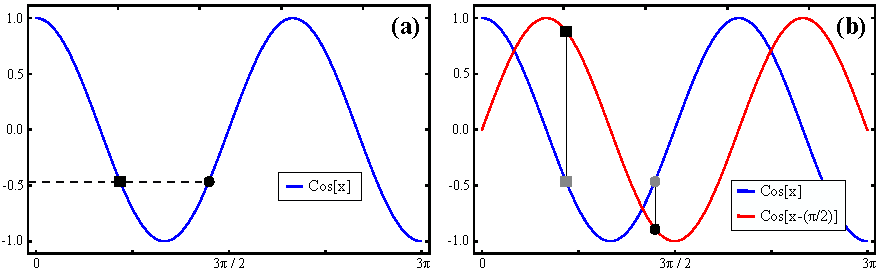
\includegraphics{figures/5/Fig_quadrature}
        \caption{\label{fig:quadrature} (a) Two points (circle, square) on a sinusoidal phase (blue curve) that are indistinguishable when measured. This limits the effective measurement range to $\pm \pi / 2$ at maximum, hence the invertible region restriction in Ramsey measurements. (b) The same two points measured with a phase shift of $\pi / 2$ (red curve). The addition of this phase shifted measurement distinguishes the two points and extends the measurement range to $\pm \pi$. This is also called a quadrature measurement. }
    \end{center}
\end{figure*}

To improve performance even further, the authors introduce an ``adaptive'' measurement technique \cite{BSsup}. In this method, Ramsey measurements of an ensemble are initiated as normal (a single $\pi / 2$ pulse on all atoms), but completed sequentially on subsets of the ensemble rather that on all atoms simultaneously. After a subset measurement, during which the remainder of the ensemble is still being interrogated, an intermittent adjustment can be made to the phase of the LO (not the frequency) before measuring the next subset. The subsequent measurement's outcome is therefore correlated to the first in a way which extends the invertible region beyond $\pm \pi / 2$ to $\pm \pi$, assuming that the measurements occur on a timescale $\ll T_{max}$. In principle this is similar to making a quadrature measurement, in which sampling a sinusoidal signal at both 0 and $\pi / 2$ phase offsets gives more information (Fig. \ref{fig:quadrature} (b)). The adaptive measurement method, however, involves a Bayesian analysis after each subset measurement in order to predict the LO phase shift which will maximize the sensitivity of the following measurement. 

The net result is to increase the invertible region of the error signal, and consequently increase $T_{1,max}$, for the ensemble as a whole. Specifically, the limit of $\gamma T_{1,max}$ is relaxed from 0.1 to (up to) 0.3. Subsequently, Eq. \ref{eq:clockstab} predicts $N_{min} = 4 \ (7)$ when using this protocol in the case of white ($1/f$) LO noise. 

%\begin{figure*}[t]
 %   \begin{center}
 %       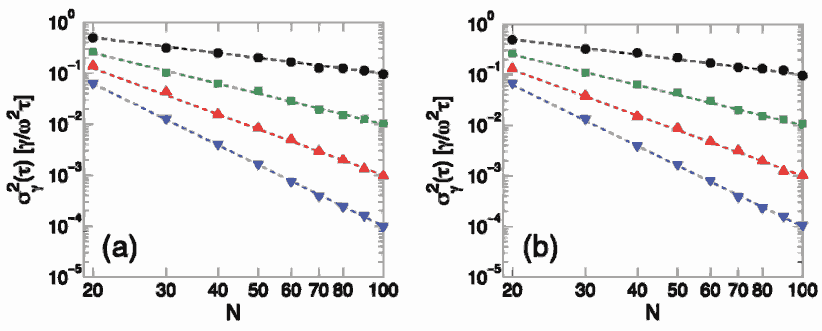
\includegraphics{figures/5/Fig3}
    %    \caption{\label{fig:adaptsim} Figures from Ref. \cite{BorregaardSorensen}. Simulated Allan variance measurements for a system of 1, 2, 3, and 4 ensembles (black, green, red, blue) of N ions. White LO noise is simulated. The simulations measure $\sigma_y^2 ({\tau})$ in the cases of (a) standard Ramsey measurements and (b) the adaptive measurements described in \cite{BSsup}.     }
   % \end{center}
%\end{figure*}








%%%%%%%%%%%%%%%%%%%%%%%%

\section{Implementation in a $^{40}$Ca$^+$ optical clock}

Our primary long-term goal in this project is to improve LO performance in a trapped ion clock by implementing multi-ensemble and adaptive measurement techniques. We believe that such a clock will be an excellent candidate for the basis of small-scale, portable frequency references. Decreased LO quality is one of the primary technical hurdles in building a high performance small-scale device, particularly one based on an optical reference frequency as lasers are usually stabilized to large, heavy glass cavities. A clock based on our $^{40}$Ca$^+$ system already has several advantages when considering adaptations to small-scale device: First, choosing the suitably narrow $S_{1/2} \leftrightarrow D_{5/2}$ transition as the reference means that the interrogating LO will be the 729 nm laser, which is in the optical frequency range ($f_0 \sim 10^{14}$ Hz). The $1/f_0$ dependence in Eq. \ref{eq:shotlimit} gives optical clocks\footnote{A good overview of optical clocks is provided in Ref. \cite{OpticalClocks}.} a natural advantage in stability over microwave frequency clocks such as caesium standards, which have $f_0 \sim 10^9 - 10^{10}$ Hz. Despite there being probeable atomic transitions with substantially greater frequencies than those in the optical range, such as M\"{o}ssbauer transitions on the order of $10^{19}$ Hz \cite{OpticalClocks}, LOs in the optical range meet the requirements of 1) being producible with a sufficiently narrow linewidth, due to the development of lasers and cavity-based stabilization \cite{StableLaser1, 6174186,McFerran:12,KesslerT.2012,Y.2011,PhysRevA.79.053829,Dubé2009,Ludlow:07, PhysRevLett.82.3799} and 2) having countable cycles, due to the development of optical frequency combs \cite{R.2008,RevModPhys.78.1297,Grosche2008,RevModPhys.78.1279,RevModPhys.75.325,Udem:99, PhysRevLett.88.073601,PhysRevLett.84.5102}. A particular advantage to using $^{40}$Ca$^+$  is that many other ion species only have suitable optical transitions in the UV range, which are not as easily producible. Second, planar ion traps like the one used in this work already have demonstrated scalability (the Gen IIc for instance is already on the order of 1 cm$^2$). Third, although fewer atoms will participate in the clock measurement than in thermal vapor or optical lattice based devices, a clock based on trapped/cooled ions have longer coherence times (see next section) and will therefore allow longer interrogation times, increasing the overall sensitivity per atom/ion. 

For realizing a multi-ensemble clock, we must be able to load and confine multiple ions. This is already within the capabilities of our Gen IIc trap, which has previously demonstrated a single linear chain of 10 ions \cite{IonTrap}. A similar GTRI planar trap in our lab has recently loaded 35 ions in a single linear chain, so there is room yet for improvement in our system. The ability to separate chains into multiple ensembles or subsets of ensembles is inherent to the design of our traps and is used for deterministic loading and to perform quantum gates \cite{Kielpinski2002}. 

For performing adaptive measurements, we must be able to interrogate and measure individual ions or subsets in an ensemble. There are several options available to us in our system, each with different merits. First, our use of an optical frequency LO and state-detection beam makes single-ion addressing possible, since focused beam waists can be realized that are several times less than the typical ion spacing in a linear chain ($\sim$ 3-7 $\mu$m). Precision beam-steering can be technically challenging to implement, however. An alternative to single-ion addressing involves separating a subset of ions from a larger chain and transporting them to a location where they can be independently interrogated/measured. This requires that transport operation be performed within the timescale of both the overall interrogation time and the state coherence time of the ions. Finally, arbitrary state rotations can also be achieved by dynamically transporting an ion through a static, steady-state beam \cite{TransGateTh,TransGateExp}. Because high-speed beam pulsing typically requires the use of AOMs and their peripheral hardware, this so-called transport method of state control is advantageous in that it does not require this additional hardware overhead. However, achieving the precise transport necessary for this method can be technically challenging. 




%%%%%%%%%%%%%%%%%%%%%%%%%%%%

\section{Research goals}


%%%%%%%%%%%%%%


\begin{figure*}[hp]
    \begin{center}
        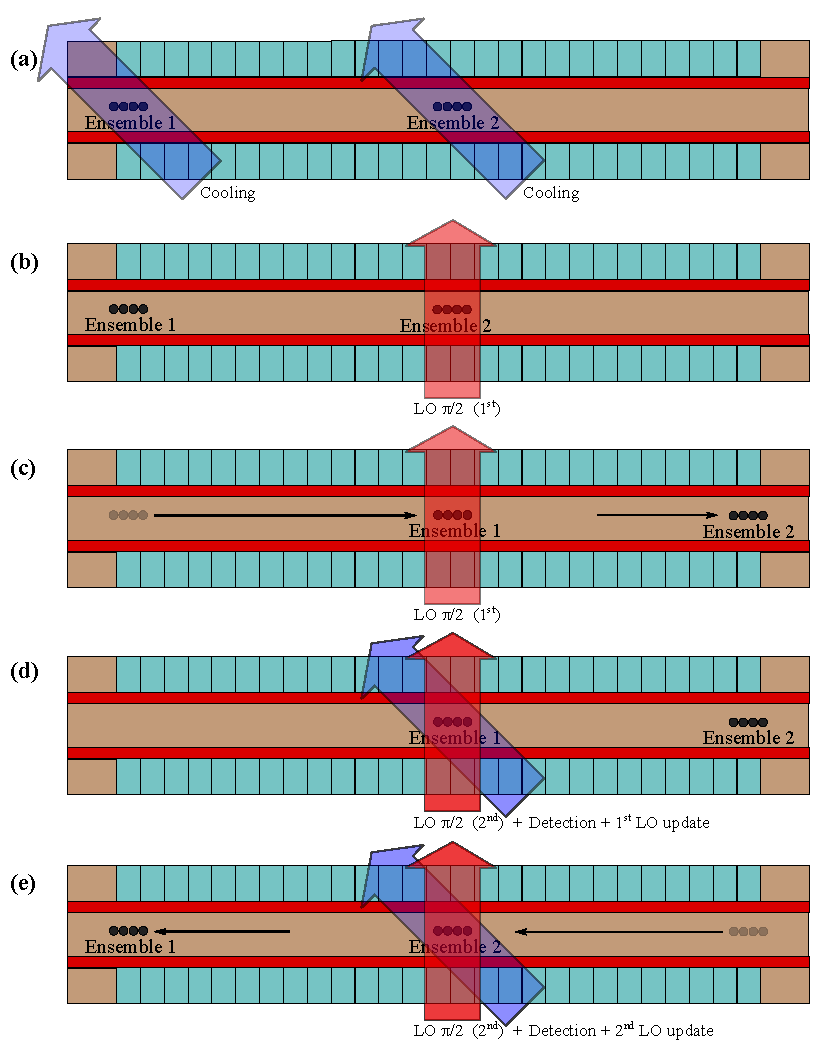
\includegraphics{figures/5/Fig_ClockScheme2}
        \caption{\label{fig:clockscheme} A possible scheme for a 2-ensemble clock in our system. (a) Ensembles 1 and 2 are initialized and cooled. (b) Ensemble 2 receives the first $\pi / 2$ pulse of a Ramsey measurement. (c) Ensemble 2 is transported away and begins its interrogation period; Ensemble 1 is transported in, receives its first $\pi / 2$ pulse, and free-evolves for $T_1 \leq T_{1,max}$. (d) Ensemble 2 continues to free-evolve; Ensemble 1 receives its second $\pi / 2$ pulse, followed by a state detection and update to the LO frequency. (e) Ensemble 1 is transported back to its beginning point; Ensemble 2 completes its interrogation period $T_2 \leq T_{2,max}$ and is transported back to its start point. A final $\pi /2$ pulse and state detection occurs, and the LO is updated again. The entire cycle now repeats. Adding adaptive measurements simply involves intermittent steps after (c) to divide the ensembles into appropriate subsets.   }
    \end{center}
\end{figure*}

Fig. \ref{fig:clockscheme} shows a potential scheme for how a 2-ensemble clock with adaptive measurements could be realized in our ^{40}$Ca$^+$ system. This scheme uses ion/subset transport for interrogating/measuring multiple ensembles. Successful implementation will have several key technical requirements: first, we must show that ion coherence times in our system are not prohibitively short, both for single ions and for ensembles. Decoherence refers to the degradation of an ion's superposition state over time, due to coupling of the Hamiltonian to the external environment \cite{PhysRevA.57.3748, SACKETT2003431, RevModPhys.75.715}. Because Ramsey interrogations occur while ions are in a superposition state of the reference transition, decoherence will limit achievable interrogation times. Although we have previously measured single-ion coherence times of $\sim$ 1-1.5 ms in our system, which is generally sufficient for basic clock operation, the scheme in Fig. \ref{fig:clockscheme} includes transport operations which must be performed on a similar timescale. The current stabilization cavity for the 729 nm laser should allow for 10-100 ms coherence times if all other factors are accounted for. Second, we must characterize and minimize ``state destruction'' events which occur when Ramsey superposition states experience unwanted interactions with the 397 nm laser. This can happen when scattered (or edge-of-beam) light from a state detection event reaches an ion in the middle of a Ramsey interrogation elsewhere (see Fig. \ref{fig:clockscheme} (d), for instance). 

Beyond these primary requirements, realization of our proposed scheme will include several key milestones: 1) characterizing systematic factors in our system which could cause frequency shifts in a clock (magnetic field noise, for instance), 2) configuring the our system to function as a simple frequency reference for the 729 nm laser, 3) configuring the system to load, merge, and separate multi-ion ensembles, 4) demonstrating coherent transport of whole ensembles, and 5) performing rapid phase updates to the 729 nm LO during adaptive measurements. Once we have successfully implemented this scheme with a pulsed interrogation beam, we can consider implementing the transport method for ion interrogations instead. 












%%%%%%%%%%%%%%%%%%%%%%%%%%%%%%%%%%%%%%%%%%%%%%%%%

\section{Preliminary results}

In this section we will discuss and show results from preliminary efforts towards realizing a 2-ensemble clock with adaptive measurements in our system. Our focus has been primarily to characterize the key technical aspects of ion decoherence, transport, and state destruction. 

%\subsection{Characterization of systematic frequency shifts}



\subsection{Coherence times of a single ion}

\begin{figure*}[t]
    \begin{center}
        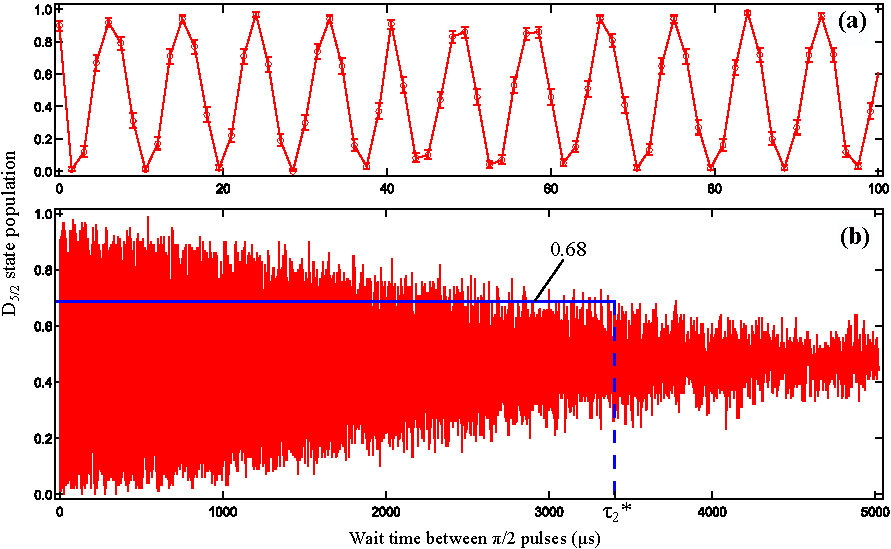
\includegraphics{figures/5/Fig_CoherenceTime2}
        \caption{\label{fig:coherencetime} $D_{5/2}$ populations measured after 2 separate $\pi / 2$ pulses, with a varying wait time between them. Both pulses have the same relative phase set by the laser. (a) The population measurements oscillate at twice the detuning frequency between the ion and the 729 nm laser (about 4 kHz here). (b) The same data over a broader time scale. The overall amplitude of these oscillations decays in time due to decoherence of the ion's superposition state. The coherence time $\tau_2^*$ is defined as the point when the envelope amplitude decays to $\approx 0.68$ (blue line).   }
    \end{center}
\end{figure*}

To measure the coherence time of a single sideband cooled ion ($\bar{n} \approx 0.2$), we perform 2 separate $\pi / 2$ pulses on the $S_{1/2} \rightarrow D_{5/2}$ transition, varying the wait time between them, and measure $P_e$ after the second pulse. The second pulse has the same relative phase as the first, such that $P_e (2 T_{\pi /2}) \approx 1$ when no wait time is applied. The measured $P_e$ values will take a $\sin^2$ profile as they oscillate at twice the detuning frequency between the ion and the laser (just as in a clock interrogation). Decoherence will manifest as an exponential decay in the amplitude of the oscillations over time \cite{PhysRevA.57.3748, SACKETT2003431, RevModPhys.75.715}. The characteristic coherence time $\tau_2^*$ is given by 
\begin{equation}
P_{e,max} (\tau_2^*) = \frac{1}{2} \bigg(1 + \frac{1}{e} \bigg) \approx 0.68
\end{equation}
Fig. \ref{fig:coherencetime} shows a coherence time $\tau_2^* \approx 3.4$ ms measured on the $|S_{1/2}, m_J = 1/2 \rangle \rightarrow |D_{5/2}, m_J = 1/2 \rangle$ transition in our system. In the absence of other systemic factors, we would expect to see coherence times of $\tau_2^* \sim 10-100$ set by the limit of the cavity-stabilized 729 nm linewidth of 10-100 Hz. We believe that we are limited here by either non-ideal gain settings and/or noise in the PID feedback loop \cite{doi:10.1119/1.1286663} of the cavity lock, or by phase-noise modulations introduced to the laser in a 25 m fiber optic cable, due to background mechanical/thermal stressors on the fiber \cite{Ma:94} (or some combination of the two effects). Our belief is based on 1) observed minute-to-minute sensitivity of the coherence time to the quality of the cavity locking feedback signal, 2) observing significant sensitivity in the polarization of fiber-transmitted light when the fibers are squeezed or bent, arising from phase shifts of the light in the medium, and 3) achieving transition linewidths of several hundred Hz at best, consistent with a coherence time of several milliseconds and indicative of either imperfect cavity locking or spectral broadening along the optical pathway. 

\begin{figure*}[ht]
    \begin{center}
        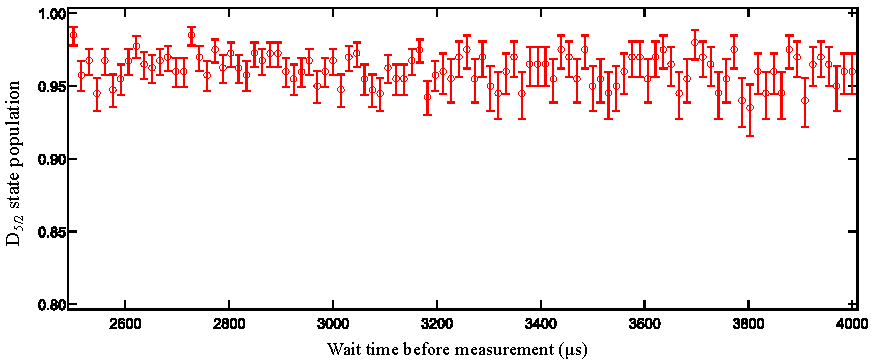
\includegraphics{figures/5/Fig_PopDecay}
        \caption{\label{fig:popflop} $D_{5/2}$ populations measured after a single inverting pulse, followed by a varying wait time. At wait times on the scale of the coherence time $\tau_2^* \approx 3.4 ms$, no significant decay in population is observed, indicating that the steady-state 866 nm laser is not causing unwanted off-resonant transitions on the 854 nm $D_{5/2} \rightarrow P_{3/2}$ transition.    }
    \end{center}
\end{figure*}

We can rule out certain other potential limiting factors in our coherence time: first, we have repeated the measurement on the $|S_{1/2}, m_J = 1/2 \rangle \rightarrow |D_{5/2}, m_J = 5/2 \rangle$ transition, which is 5 times as magnetically sensitive. We did this both with and without 60 Hz triggering of the experiments. In each case, there was no measurable difference on the coherence time, indicating that magnetic field noise effects are relatively negligible. Second, we have repeated the measurement both with and without a 1.5 ms delay added before the first $\pi / 2$ pulse. The pre-delay allows the ion undergo additional heating, on the order of that which would occur in a typical coherence time experiment. In each case, again, there was no measurable difference on the coherence time, indicating that the decay of the superposition state is not due to thermal state dephasing arising from excessive heating. Third, we have tested whether the 866 nm laser, which is continuously steady-state, was potentially causing off-resonant excitations on the 854 nm $D_{5/2} \rightarrow P_{3/2}$ transition. We did this by inverting the population to $P_e \approx 1$ in a single pulse and then measuring after a varying wait time (Fig. \ref{fig:popflop}). No decay in population over time was observed, indicating that potential off-resonant excitations are negligible if not non-existent. 



% Get that decoherence time figure in here

\subsection{Transport heating}

As described in Ch. 3, ion transport in our system is done through incremental updates to the trap's DC electrodes in order to move a harmonic well along the trap axis from point A to B. The granularity of this process will affect an ion's motional state if the transport is done in too few steps. Because our system updates electrode voltages at a rate of 10 kHz, a transport operation performed in $n$ steps will take $n \times 0.1$ ms to complete. To transport an ion within the measured coherence time of $\approx$ 3 ms, we will therefore have to limit the number of steps to $n < 30$. For a transport distance of several hundred $\mu$m or greater, this imparts a significant amount of motion to an ion in our current configuration. Beginning with $\bar{n} \approx 0.2$ sideband cooled ions, we attempted to transport ions over such distances in 15-20 steps, and measure $\bar{n}$ afterwards per Eq. \ref{eq:nbar}. However, we observed population inversions on the red sidebands begin exceed those on the blue sidebands, indicating ions that were no longer in a thermal state described by Eq. \ref{eq:Pn} and therefore rendering Eq. \ref{eq:nbar} invalid. By comparison, adiabatic transports with approximately 1 step per several $\mu$m of travel exhibit no heating beyond that of the trap's inherent heating rate. %Fig. TBD. 
% Refs about reducing heating? Ask True



\subsection{State destruction characterization}

% Branching ratio figure
State destruction occurs when an ion experiences an unwanted interaction with resonant 397 nm light during the middle of a Ramsey interrogation. To characterize state destruction, we must first understand how the resulting state measurement will have been affected. After the first $\pi /2$ pulse but before the second, the ion has an effectively equal chance of being projected into the $D_{5/2}$ or $S_{1/2}$ states by the 397 nm light. When projected into $D_{5/2}$, the second $\pi /2$ pulse of the Ramsey sequence will leave the ion back in the superposition state such that $P_e = 0.5$ on average upon measurement. This particular outcome occurs 50\% of the time on average. When projected into $S_{1/2}$, the ion will subsequently be excited on the $S_{1/2} \rightarrow P_{1/2}$ transition and then decay, with equal probability, to either the $|S_{1/2}, m_J = -1/2 \rangle$ or $|S_{1/2}, m_J = 1/2 \rangle$ ground states. Because the 729 nm LO will be tuned to excite only one of these states, the second $\pi /2$ pulse will either 1) also lead to $P_e = 0.5$ upon measurement (on average), or 2) leave the ion in the ground state, such that $P_e = 0$. Each of these respective outcomes occurs 25\% of the time on average. 


\begin{figure*}[t]
    \begin{center}
        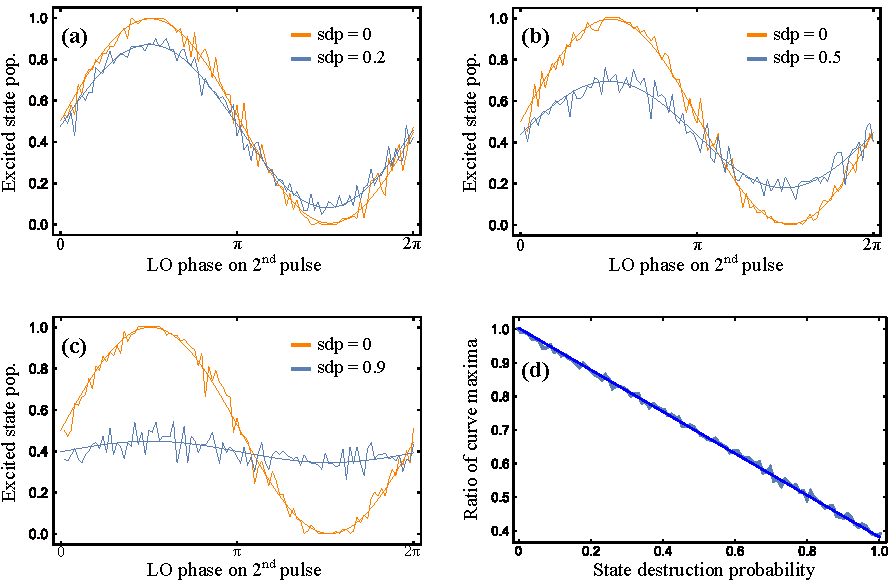
\includegraphics{figures/5/Fig_sdpsims}
        \caption{\label{fig:sdpsim} (a,b,c) Simulated Ramsey measurements with a varying phase on the second $\pi / 2$ pulse, and with state destruction probabilities of (a) 0.2, (b) 0.5, and (c) 0.9 (light blue curves). The $sdp = 0$ case is also plotted in each instance (orange curves). Each point represents the average of 100 measurement sequences (or, equivalently, 1 measurement sequence on 100 atoms). (d) The ratios of the $sdp \neq 0$ maxima to the $sdp = 0$ maxima are effectively linear in $sdp$. }. 
    \end{center}
\end{figure*}

Therefore, in the event of an unwanted interaction with 397 nm light, which we refer to as a state destruction event, the measurement outcome of the Ramsey sequence will be (on average) either $P_e = 0$ or $P_e = 0.5$, with probabilities $1/4$ and $3/4$, respectively. With this knowledge, state destruction can be numerically modeled as a probabilistic event. We consider a Ramsey measurement sequence with two resonant $\pi /2$ pulses, in which the second pulse has a varying relative phase from 0 to $2 \pi$ (as in the measurement in Fig. \ref{fig:RamseyEx} (b)). When no state destruction occurs, the measurement outcomes are probabilistic, with the excited state probability $P_e$ taking a $\sin^2$ profile as a function of the varying phase. When state destruction does occur, the measurement outcome will be $0$ or $0.5$ with probabilities $1/4$ and $3/4$, respectively. We introduce a state destruction probability parameter $sdp$ which determines the likelihood of a state destruction event taking place. Fig. \ref{fig:sdpsim} (a,b,c) shows that by varying $sdp$ from 0 to 1 in the simulation and averaging over a suitable number of measurements, the $\sin^2$ output of the Ramsey sequence gradually decays in amplitude. Each point in the data represents the average of 100 measurement sequences (or, equivalently, 1 measurement sequence on 100 atoms).

The maxima of these sinusoids relative to the $sdp = 0$ case are unique. In Fig. \ref{fig:sdpsim} (d) we measure this ratio for $0 \leq sdp \leq 1$ in increments of 0.1, and find a linear relationship. By parameterizing this relationship, we can perform these same Ramsey sequences in our experiment and quantify state destruction. Specifically, we pulse the 397 nm beam at varying distances from an ion that is between $\pi / 2$ pulses in the sequence described above, then repeat the exact same sequence with no pulse (hence $sdp = 0$ in the no-pulse instance). Fig. \ref{fig:sdp} shows these results. The pulse duration was 200 $\mu$s, which is equivalent to that of a state detection pulse in our system. The total interrogation time was just long enough to allow for the pulse to occur, minimizing decoherence. The 729 nm beam remained at a fixed position throughout ($z = 1000$ on the trap axis). 

\begin{figure*}[t]
    \begin{center}
        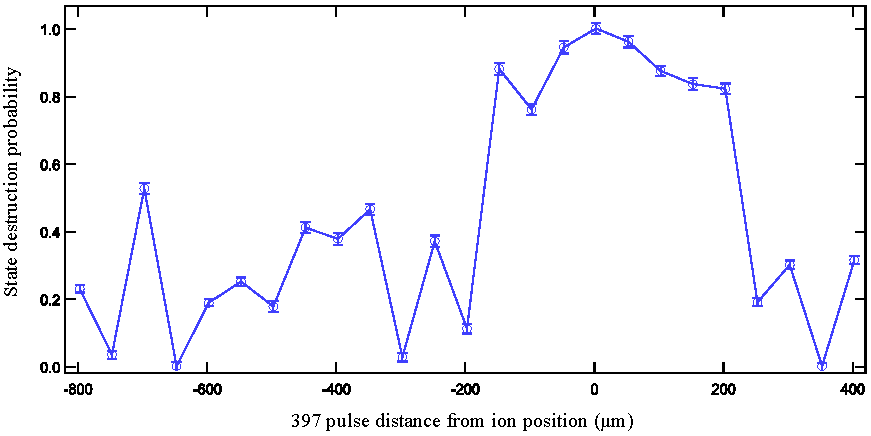
\includegraphics{figures/5/Fig_sdp}
        \caption{\label{fig:sdp} Measured state destruction probabilities in our trap vs. distance of the 397 nm beam from the ion's position ($z = 1000$). }
    \end{center}
\end{figure*}


We estimate the focused 397 nm beam waist to be 40-60 $\mu$m at the trap axis. We see in Fig. \ref{fig:sdp} that state destruction is significant within $\pm 150 \ \mu$m of the ion position, either due to significant nearby scatter from the trap surface or due to interactions with the edge of the beam profile. Beyond this range $sdp$ varies as the light scatters from the different regions of the trap, but for the most part is non-trivial throughout the range of measurement. 







%%%%%%%%%%%%%%%%%%%%%%%%
\section{Discussion}


In order to continue making progress towards a multi-ensemble clock with adaptive measurements, we will need to address these technical limitations discovered thus far. First, we will need to improve on the current single ion coherence time of $\approx$ 3 ms in order to allow for suitably adiabatic transport operations. Improvements to the laser's cavity stabilization can be made through precise calibrations of the PID loop's gain settings, as well as from performing a systematic analysis of any noise which may exist in the feedback signal. Previous experiments in our lab have not required coherence times longer than what we have measured, so it likely that improvements can be made to the cavity lock which were previously unnecessary. Output linewidths approaching 10 Hz should be possible in this cavity, given its finesse. Phase-noise modulation of the laser due to stress on the optical fiber(s) can be reduced by implementing a method demonstrated in Ref. \cite{Ma:94}, in which a portion of the transmitted light is reflected back through the fiber and measured against the input light, allowing the phase difference to be monitored and continuously corrected during experiments. Using this method, the authors reduce the linewidth of 532 nm light transmitted through a 25 m optical fiber from 1.2 kHz to 16 Hz, with only a marginal reduction in carrier power. Assuming no other contributing factors, a similar reduction in linewidth in our system would achieve 50-100 ms coherence times, which should be suitable for adiabatic transport during clock cycles.

Beyond extending the single-ion coherence time, we will need to measure the coherence times for multi-ion ensembles and ensure that they are also suitable for transport. Upgrading the system's digital-to-analog converters would also increase the electrode update rate of 10 kHz and allow for faster transport operations. In Ref. \cite{PhysRevLett.109.080502}, converters with an update rate of 50 MHz were used to diabatically transport single ions and separate two-ion chains on timescales of 10-50 $\mu$s, with overall heating $<$ 2-3 quanta. 

In order to address and reduce state destruction in our system, there are several improvements which can be made easily and immediately. The first would be to reduce the focused waist of the 397 nm detection beam, which will reduce light scatter. A waist of 10-15 $\mu$m is easily achievable for this wavelength with appropriate optics, and would still allow for simultaneous addressing of 4-6 ions in an ensemble. The second would be to better isolate the PMT from ambient room light, which will increase detection efficiencies and allow us to use shorter detection pulses, further reducing the chances of state destruction events. Detection efficiencies of 99.99\% have been demonstrated for both single $^{40}$Ca$^+$ ions and ensembles of 4 \cite{PhysRevLett.100.200502, PhysRevA.81.040302}.  Once these improvements are made, the experiment in Fig. \ref{fig:sdp} can be repeated in the updated configuration, with greater spatial resolution and with varying placements of the 729 nm beam. Thorough knowledge of the state destruction probabilities which occur for the different beam placements will allow us to choose the best ensemble and beam positions in Fig. \ref{fig:clockscheme}. 

% \textit{Blab about simulations?} Even if state destruction cannot be eliminated entirely during ensemble interrogations










